\section[Vererbung]{Vererbung \tiny{Kap. 23}}

\begin{minipage}[t]{0.64\textwidth}
	\begin{itemize}
		\item eine neue Klasse aus einer bestehenden Klasse ableiten:
		\item \textbf{Person} ist eine:\\
		Oberklasse, Basisklasse, Elternklasse oder Superklasse
		\item \textbf{Angestellter} und \textbf{Bürger} sind eine:\\
		Unterklasse, abgeleitete Klasse, Kindklasse oder Subklasse
	\end{itemize}
\end{minipage}
\hspace{0.02\textwidth}
\begin{minipage}[t]{0.34\textwidth}
	$\quad$\\
	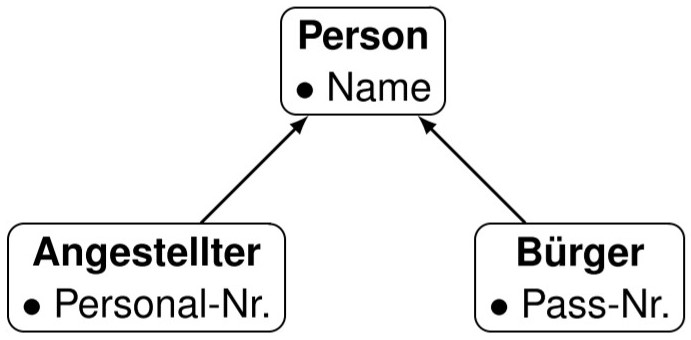
\includegraphics[width=\textwidth]{images/v7_vererbung1}
\end{minipage}

\lstinputlisting{listings/v7_vererbung5.py}



\begin{minipage}[t]{0.49\textwidth}
	\subsection{Beispiel}
	\lstinputlisting{listings/v7_vererbung6.py}
\end{minipage}
\hspace{0.02\textwidth}
\begin{minipage}[t]{0.49\textwidth}
	$\quad$\\
	Die Person-Klasse instanzieren:
	\lstinputlisting{listings/v7_vererbung7.py}
\end{minipage}\\[12pt]

\begin{minipage}[t]{0.49\textwidth}
	Angestellte-Klasse erbt von der Person-Klasse:\\
	\lstinputlisting{listings/v7_vererbung8.py}
\end{minipage}
\hspace{0.02\textwidth}
\begin{minipage}[t]{0.49\textwidth}
	Die Angestellter-Klasse instanzieren:\\
	\lstinputlisting{listings/v7_vererbung9.py}
\end{minipage}


\begin{minipage}[t]{0.49\textwidth}
	$\quad$\\[20pt]
	
	\subsection{\texttt{public}, \texttt{protected} und \texttt{private}}
	Die Konvention ist wie folgt:
	\begin{description}
		\item[\texttt{public:}] für für öffentliche Variablen und Methoden
		\item[\texttt{protected:}] (1 führender Unterstrich) für nicht-öffentliche Variablen und Methoden
		\item[\texttt{private:}] (2 führende Unterstriche) für nicht-öffentliche Variablen und Methoden, um Namenskonflikte in Subklassen zu vermeiden 
	\end{description}
	\url{https://www.python.org/dev/peps/pep-0008/#method-names-and-instance-variables}
\end{minipage}
\hspace{0.02\textwidth}
\begin{minipage}[t]{0.49\textwidth}
	\lstinputlisting{listings/v7_vererbung10.py}
\end{minipage}


\begin{minipage}[t]{0.49\textwidth}
	\section[Mehrfachvererbung]{Mehrfachvererbung \tiny{Kap. 24}}
	Eine Subklasse kann von mehreren Superklassen erben:\\
	\begin{minipage}[t]{0.54\textwidth}
		\lstinputlisting{listings/v7_vererbung11.py}
	\end{minipage}
	\begin{minipage}[t]{0.02\textwidth}$\quad$\end{minipage}
	\begin{minipage}[t]{0.4\textwidth}
			$\quad$\\[18pt]
			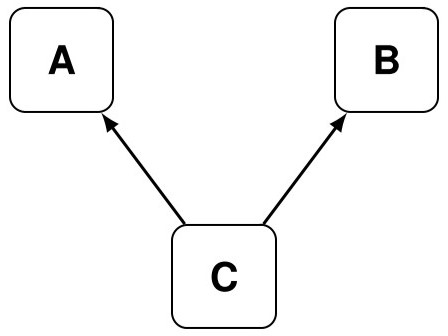
\includegraphics[width=\textwidth]{images/v7_vererbung2}
	\end{minipage}
	
	Am besten die \texttt{\_init\_\(\)}-Methode der Klassen kooperativ machen, d.h.
	\begin{itemize}
		\item immer \texttt{super()} benutzen
		\item Schlüsselwort-Argumente benutzen
		\item unbenutzte Schlüsselwort-Argumente weitergeben (\texttt{**kwargs})
		\item \texttt{super()} ruft automatisch die Methode der nächsten Klasse auf
		\item Method Resolution Order (MRO) $\rightarrow$ C4 Superclass Linearization (\url{https://en.wikipedia.org/wiki/C3_linearizatio})
		\item Diamond-Problem ist kein Problem mit \texttt{super()}
	\end{itemize}
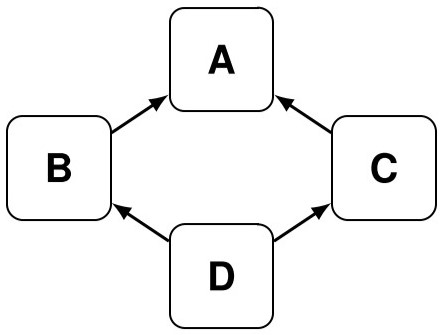
\includegraphics[width=0.5\linewidth]{images/v7_vererbung3}
\end{minipage}
\hspace{0.02\textwidth}
\begin{minipage}[t]{0.49\textwidth}
	\lstinputlisting{listings/v7_vererbung12.py}
\end{minipage}


\subsubsection{MRO}
\begin{minipage}[t]{0.49\textwidth}
	Mehrfachvererbung in Diamant-Anordung:
	\lstinputlisting{listings/v7_vererbung13.py}
\end{minipage}
\hspace{0.02\textwidth}
\begin{minipage}[t]{0.49\textwidth}
	\texttt{\textbf{super()}} ruft die Methoden der Reihe nach auf:
	\lstinputlisting{listings/v7_vererbung14.py}
	Die Reihenfolge wird vom MRO-Algorithmus festgelegt:
	\lstinputlisting{listings/v7_vererbung15.py}
\end{minipage}

